\documentclass[12pt, letterpaper, twoside]{article}
\usepackage[T2A]{fontenc}
\usepackage{amsfonts}
\usepackage{amsmath}
\usepackage{mathabx}
\usepackage{graphicx}
\usepackage{tikz}

\title{Семинары по дискретной математике модуль 4}
\author{Андрей Тищенко}
\date{2023/2024 гг.}

\begin{document}
    \maketitle
    \[\textbf{Семинар 4 апреля}\]
    \[\text{Графы}\]
    $G = (\underset{\neq \emptyset}{V},\ E);\ \begin{cases}
        1. E \subseteq V^2\\
        2. E\text{ иррефлексивно}\\
        \forall x \neg\ xEx\\
        3. E\text{ симметрично}\\
        \forall x,\ y (xEy\Rightarrow yEx) 
    \end{cases}$
    \begin{enumerate}
        \item[Вопрос 1.] $V = \underline{n}$. Сколько существует различных графов на $V$?\\
        Для графа размера 3.\\
        Количество неупорядоченных пар различных вершин = $|\mathcal{P}_2(V)| = C_3^2 = 3$\\
        Количество способов выбрать ребра = $|\mathcal{P}(\mathcal{P}_2(V))| = 2$\\
    \end{enumerate}
    $\{x,\ y\}$ - ребро $\Leftrightarrow xEy \wedge yEx$
    \[\text{Степенная последовательность}\]
    \begin{enumerate}
        \item[2.] $(3,\ 3,\ 2,\ 2,\ 2,\ 2)$\\
        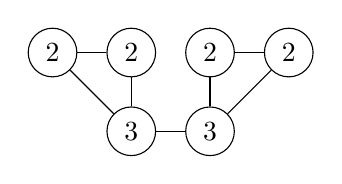
\begin{tikzpicture}[main/.style = {draw, circle}] 
            \node[main] (1) {$3$};
            \node[main] (2) [right of=1] {$3$};
            \node[main] (3) [above of=2]{$2$};
            \node[main] (4) [right of=3]{$2$};
            \node[main] (5) [above of=1]{$2$};
            \node[main] (6) [left of=5]{$2$};
            \draw (1) -- (2);
            \draw (1) -- (5);
            \draw (5) -- (6);
            \draw (1) -- (6);
            \draw (2) -- (3);
            \draw (3) -- (4);
            \draw (2) -- (4);
        \end{tikzpicture}
    \end{enumerate}
        \[\text{Лемма о рукопожатиях}\]
        $(n,\ m)\text{ - граф } G = (V,\ E)\\
        \displaystyle \sum_{x \in V} d_G(x) = 2m = |E|$
        \begin{enumerate}
            \item[3.] $(4,\ 4,\ 4,\ 4,\ 2)$ не является степенной.
            \item[4.] Задача
            \begin{enumerate}
                \item[Дано:] $(n,\ m)$ граф, $G = (V,\ E),\ n\geq 2$
                \item[Хотим:] $\exists x,\ y\in V\ \big(x\neq y \wedge d(x) = d(y)\big)$\\
                $\forall x\ 0 \leq d(x) \leq n - 1\quad d(x)\in \underline{n}$\\
                \item[Псуть не так:] $\Rightarrow d$ инъективна.\\
                $\underline{n}\sim V\overset{d}{\lesssim} \underline{n}\Rightarrow d$ сюръективна $\Rightarrow \begin{cases}\exists x_0\ d(x_0) = 0 \\ \exists x_{n - 1}\ d(x_{n - 1}) = n - 1\end{cases}$\\
                $\neg x_0 E x_{n - 1}\\
                \forall y\ (y \neq x_{n - 1})\Rightarrow x_{n - 1}Ey\Rightarrow x_{n - 1}Ex_0\Rightarrow \bot$
            \end{enumerate}
            \item[5.] Хотим построить граф со степенной последовательностью $(2,\ 2,\dots,\ 2)$\\
            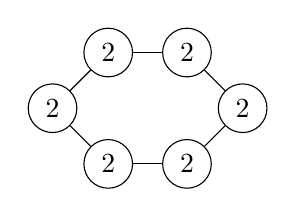
\begin{tikzpicture}[main/.style = {draw, circle}]
                \node[main] (1) {$2$};
                \node[main] (3) [right of = 1] {$2$};
                \node[main] (4) [above left of = 1] {$2$};
                \node[main] (2) [above right of = 4] {$2$};
                \node[main] (5) [above right of = 3] {$2$};
                \node[main] (6) [above left of = 5] {$2$};
                \draw (1) -- (3);
                \draw (2) -- (4);
                \draw (4) -- (1);
                \draw (3) -- (5);
                \draw (5) -- (6);
                \draw (2) -- (6);
            \end{tikzpicture}
            Граф $C_6\ncong C_3 \sqcup C_3$
            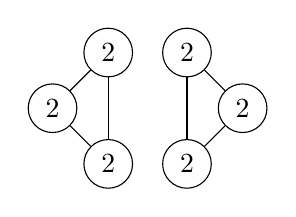
\begin{tikzpicture}[main/.style = {draw, circle}]
                \node[main] (1) {$2$};
                \node[main] (3) [right of = 1] {$2$};
                \node[main] (4) [above left of = 1] {$2$};
                \node[main] (2) [above right of = 4] {$2$};
                \node[main] (5) [above right of = 3] {$2$};
                \node[main] (6) [above left of = 5] {$2$};
                \draw (2) -- (4);
                \draw (4) -- (1);
                \draw (3) -- (5);
                \draw (5) -- (6);
                \draw (2) -- (1);
                \draw (3) -- (6);
            \end{tikzpicture}\\
            Пусть в $G $ ровно $ k$ компонент связности. Одна компонента порядка $n_i \leq n,\ n_i = 5\\
            (\underset{n_i}{\underbrace{2,\ 2,\dots,\ 2}})\Rightarrow G \cong C_{n_1}\sqcup\dots \sqcup C_{n_k},$ где $\forall i\ n_i\geq 3,\ n_1 + \dots + n_k = n\\
            1 \leq k \leq \dfrac{n}{3}$ (округлить вверх)
            \item[7.] $(100,\ 800)$ граф $G = (V,\ E)$
            \begin{enumerate}
                \item[a.] $\forall x\ d_G(x) < 16?$ Неверно по лемме о рукопожатиях.
                \item[б.] $\forall x\ d_G(x) = 16$.
                \item[Определение:] граф называют $\underline{\text{r-регулярным}}\Leftrightarrow \forall x\ d(x) = r$. Размер\\
                $r$-регулярного графа на $n$ вершинах есть $\dfrac{rn}{2}$.\\
                $K_{t + 1}$ - заведомо $t$-регулярный граф (полный граф на $t + 1$ вершине).\\
                Для нашей задачи возьмём $K_{17}$. В нём будет $\dfrac{17\cdot 16}{2} = 136$ рёбер.\\
                $800 = 136\cdot 5 + 120\\
                G \overset{?}{=} 5K_{17} + G'$, где $G'$ 16-регулярный $(15,\ 120)$ граф (такого не бывает, так как одна из 15 вершин должна быть соседом с 16 другими $\bot$). Запрашиваю продолжение конспекта, тяжело.
            \end{enumerate}

        \end{enumerate}
        \[\textbf{Семинар 11 апреля}\]
        \begin{enumerate}
            \item[7. б.] 16 регулярный граф на 100 вершинах.\\
            $V = 100,\ xEy \Leftrightarrow \exists z\in \{\pm 8,\ \pm 7,\dots,\ \pm 1\} = U\quad \big(x - y\equiv z\ (100)\big)$.\\
            $E$ иррефлексивно.
            \[xEx \Rightarrow x - x = 0 \equiv z (100)\Rightarrow \bot\]
            Симметричность.
            \[xEy \Rightarrow yEx\]
            \[\exists z \in U\quad x - y \equiv z\ (100)\Rightarrow \begin{cases}
                y - x \equiv -z (100)\\
                -z \in U
            \end{cases}\Rightarrow yEx\]
            $x\in \underline{100}.\ N(x) = \{(x - 8),\ (x - 7),\dots,\ (x - 1),\ (x + 1),\dots,\ (x + 8)\}$\\
            Почему среди них нет одинаковых? Пусть есть:\\
            $(x + d_1)\% 100 = (x + d_2)\% 100,\ |N(x)|\leq 16\\
            \Leftrightarrow x + d_1 \equiv x + d_2\ (100)\\
            \Leftrightarrow d_1 \equiv d_2\ (100) \Rightarrow \exists k\in \mathbb{Z}\quad |d_1 - d_2| = 16k\wedge d_2 - d_1 \leq 16\Rightarrow\\
            \Rightarrow d_1 = d_2 = 0$.
            \item[8.] Среди любых шестерых людей есть хотя бы трое незнакомых или хотя бы трое знакомых.\\
            Пусть есть такая вершина, что у него есть три соседа.
            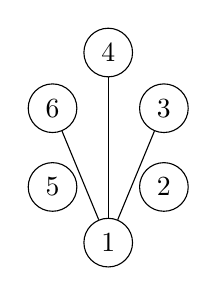
\begin{tikzpicture}[main/.style = {draw, circle}]
                \node[main] (1) {$1$};
                \node[main] (2) [above right of=1] {$2$};
                \node[main] (3) [above of=2]{$3$};
                \node[main] (4) [above left of=3]{$4$};
                \node[main] (5) [above left of=1]{$5$};
                \node[main] (6) [above of =5]{$6$};
                \draw (1) -- (3);
                \draw (1) -- (4);
                \draw (1) -- (6);
            \end{tikzpicture}
            Между вершинами $3,\ 4,\ 6$ может быть ребро, тогда есть три попарно знакомых, может не быть рёбер, тогда есть три попарно незнакомых.
            \item[9.] Булев куб:\\
            $x_1,\dots,\ x_n E y_1,\dots,\ y_n\Leftrightarrow \exists i\ (x_i \neq y_i \wedge \forall j \neq 1\ x_j = y_j)$\\
            $n = 1$\\
            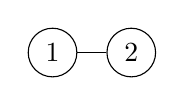
\begin{tikzpicture}[main/.style = {draw, circle}]
                \node[main] (1) {$1$};
                \node[main] (2) [right of=1] {$2$};
                \draw (1) -- (2);
            \end{tikzpicture}\\
            $n = 2$\\
            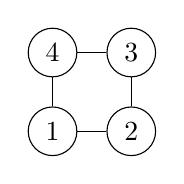
\begin{tikzpicture}[main/.style = {draw, circle}]
                \node[main] (1) {$1$};
                \node[main] (2) [right of=1] {$2$};
                \node[main] (3) [above of = 2] {$3$};
                \node[main] (4) [left of = 3] {$4$};
                \draw (1) -- (2);
                \draw (2) -- (3);
                \draw (3) -- (4);
                \draw (1) -- (4);
            \end{tikzpicture}\\
            $n = 3$. Тут куб, поверьте, пожалуйста.
            \begin{enumerate}
                \item[a.] $|V_n| = 2^n$
                \item[b.] Число рёбер графа $B_n$ = $2^n\cdot \frac{n}{2} = 2^{n - 1} n$
                \item[c.] $2^n \cdot C^2_n$ 
            \end{enumerate}
        \end{enumerate}
        \[\text{Дополнение графа.}\]
        $G = (V,\ E),\quad \overline{G} = \big( V,\ (V^2\setminus \operatorname{id}_V)\setminus E \big)$
        Нарисуем дополнение:\\
        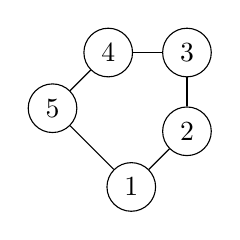
\begin{tikzpicture}[main/.style = {draw, circle}]
            \node[main] (1) {$1$};
            \node[main] (2) [above right of=1] {$2$};
            \node[main] (3) [above of=2]{$3$};
            \node[main] (4) [left of=3]{$4$};
            \node[main] (5) [below left of=4]{$5$};
            \draw (1) -- (2);
                \draw (2) -- (3);
                \draw (3) -- (4);
                \draw (4) -- (5);
                \draw (5) -- (1);
        \end{tikzpicture}\\
        Дополнением к такому графу будет граф\\
        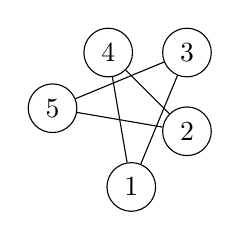
\begin{tikzpicture}[main/.style = {draw, circle}]
            \node[main] (1) {$1$};
            \node[main] (2) [above right of=1] {$2$};
            \node[main] (3) [above of=2]{$3$};
            \node[main] (4) [left of=3]{$4$};
            \node[main] (5) [below left of=4]{$5$};
            \draw (1) -- (4);
            \draw (2) -- (5);
            \draw (3) -- (1);
            \draw (4) -- (2);
            \draw (5) -- (3);
        \end{tikzpicture}\\
        Докажем $G$ не связен $\Rightarrow \overline{G}$ связен.\\
        Рассмотрим произвольные вершины $x,\ y\ (x\neq y) \in V$.\\
        Первый случай: $x \nsim_G y \Rightarrow \neg xEy\Rightarrow x\overline{E}y$\\
        Второй случай: $x \sim_G y$, так как $G$ не связен, то $\exists w: \begin{cases}
            x \nsim_G w\\
            y \nsim_G w
        \end{cases}\Rightarrow\\ \Rightarrow xw,\ yw \notin E\Rightarrow xw,\ yw \in \overline{E}\Rightarrow x \sim_{\overline{G}} y$ 
        \begin{enumerate}\newpage
            \item[11.] Доказать:\\
            $\left. \begin{matrix}
                (n,\ m)\text{ - граф }G\\
                n = 15\\
                \forall x\ d(x) \geq 7
            \end{matrix} \right|\Rightarrow G\text{ связен} $\\
            Рассмотрим произвольные $x$ и $y$ и допустим $x\nsim y\Rightarrow (xy \notin E)\\
            \Leftrightarrow \begin{cases}
                x \notin N(x) \cup N(y)\\
                y \notin N(x) \cup N(y)
            \end{cases}$\\
            $N(x) \cup N(y) \subseteq V\setminus \{x,\ y\}\\
            |N(x)| + |N(y)| = |N(x) \cup N(y)|\leq 15 - 2 = 13$\\
            Так как $|N(x)| \geq 7 \wedge |N(y)| \geq 7\Rightarrow 7 + 7 - |N(x) \cap N(y)|\leq 13\Rightarrow\\
            \Rightarrow N(x)\cap N(y)\neq \emptyset$
        \end{enumerate}
    \[\textbf{Семинар 18 апреля}\]
    \begin{enumerate}
        \item[Задача 12.] Уединённая $\Rightarrow$ степень не больше 3. Каждая вершина соединена хотя бы с тремя уединёнными.\\
        Возьмём любую вершину $x$. У неё должно быть хотя бы $3$ уединённых соседа, пусть среди них есть уединённая вершина $y$. У любой уединённой вершины степень не больше 3 и она имеет хотя бы 3 уединённых соседа, значит все её соседи являются уединёнными, то есть вершина $x$ является уединённой. Получается, что любая вершина является уединённой.\\
        Построим такой граф на 100 вершинах. Можно привести в приимер 25 полных графов на $4$ вершинах
        \item[Задача 13.] 1 случай. Если граф полный, то очевидно
        2 случай. Граф не полный $G \ncong K_n,\ n\geq 4\Rightarrow \exists x,\ y\ \neg xEy$\\
        $|N(x)|\geq \frac{n}{2};\ |N(y)| \geq \frac{n}{2}\\
        |N(x) \cup N(y)| \leq n - 2$, так как $x,\ y\notin N(x) \wedge x,\ y \notin N(y)\Rightarrow\\
        \Rightarrow x,\ y\notin N(x)\cup N(y)$
        $|N(x) \cup N(y)| = |N(x)| + |N(y)| - |N(x)\cap N(y)|\\
        |N(x)| + |N(y)| \geq n \Rightarrow n - 2 \geq n - |N(x) \cap N(y)|\Rightarrow |N(x) \cap N(y)| \geq 2\Rightarrow \exists u,\ v$ (вершины), такие что:\\
        $xEv \wedge vEy \wedge yEu \wedge uEx\cong C_4$, ч.т.д.
    \end{enumerate}
    Утверждение 1: если $(n,\ m)$ - граф $G$ связен, то $m \geq n - 1$\\
    Утверждение 2: $\forall (n,\ m)$ - графа $G$, $m \leq C^2_n$\\
    Утверждение 3: Если $G$ не связен, то $\overline{G}$ связен (см. задачу 10)\\
    Утверждение 4: $\forall (n,\ m)$ - графа $G$. $\overline{G}$ есть $(m,\ C_n^2 - m)$ - граф
    \begin{enumerate}
        \item[Задача 14.] Допустим есть несвязный $(n,\ m)$ - граф $G$. Тогда связно его дополнение, являющееся $(n,\ C_n^2 - m)$ граф $\overline{G}$, значит для него выполнятеся $C_n^2 - m \geq n - 1\Rightarrow \dfrac{n(n - 1)}{2} - m \geq n - 1\Rightarrow m \leq (n - 1)(\frac{n}{2} - 1)\Rightarrow\\
        \Rightarrow m \leq \dfrac{(n-  1)(n - 2)}{2} = C^2_{n - 1}$
    \end{enumerate}
    Утверждение 5: Если $(n,\ m)$ - граф $G$ не связен, то $m \leq C^2_{n - 1} < C^2_n$. Эта оценка неулучшаема (оптимальна). Это означает, что:\\
    $\forall n \geq 2\ \exists$ несвязный $(n,\ C^2_{n - 1})$ - граф $G$
    \begin{enumerate}
        \item[Задача 15.] Пусть есть две вершины $x \neq y$ степени 5.\\
        1 случай. Пусть они смежные (то есть $xEy$). Рассмотрим вершины, с которыми они связаны. Рассмотрим $\big(N(x)\setminus \{y\}\big) \cap \big( N(y) \setminus \{x\}\big)\\
        |N'(x)| = |N(x)\setminus \{y\}| = |N(y)\setminus \{x\}| = N'(y) = 5 - 1 = 4\Rightarrow\\
        \Rightarrow |N'(x) \cup N'(y)| \leq |V_G| - 2 = 9 - 2 = 7\Rightarrow |N'(x) \cap N'(y)|\geq 1\Rightarrow$ есть цикл. Противоречие.\\
        2 случай. $x,\ y \notin N(x) \cup N(y)\\
        |N(x) \cup N(y)| \leq 9 - 2=  7\\
        \underset{=10}{2|N(x)|} - |N(x)\cap N(y)|\\
        |N(x)\cap N(y)| \geq 3\Rightarrow$ найдётся цикл.
        \item[Задача 16.] $n\geq 2 \wedge m = n - 1$\\
        Лемма о рукопожатиях: $2(n - 1) = \displaystyle \sum_{x \in V} d(x)$\\
        Пусть $t :=$ число вершин степени 1.\\
        Тогда $2(n - 1) = \displaystyle \sum_{x\in V \wedge d(x) \geq 2} d(x) + t$. Хотим $t \geq 2$\\
        Заметим $\displaystyle \sum_{x\in V} d(x) \geq 2(n - t)$. То есть\\
        $2(n - 1) \geq 2(n - t) + t\\
        2n - 2(n - 1) \leq t\Rightarrow 2 \leq t$ ч.т.д.
        \item[Задача 17.] Число вершин степени $2 = 0$, степени $1 = t$\\
        $2(n - 1) = \displaystyle\sum_{x \in V} d(x) = t + \sum_{x \in V\wedge d(x) \geq 3}d(x)$\\
        $2(n - 1) \geq t + 3(n - t)\Rightarrow 2n - 2 \geq t + 3n - 3t\Rightarrow \\
        \Rightarrow -n - 2 \geq -2t\Rightarrow t \geq \dfrac{n + 2}{2} = \dfrac{n}{2} + 1 > \dfrac{n}{2}$, ч.т.д.
        \item[Задача 18.] Возьмём остовное дерево в нашем графе. В любом дереве с количеством вершин более 2 есть хотя бы две вершины степени 1, можно удалить любую из них. Если вершина одна, то связность при удалении не потеряется.
    \end{enumerate}
    \[\textbf{Семинар 25 апреля}\]
    \begin{enumerate}
        \item[Задача 19.] Проверить какой-нибудь граф на двудольность.
    \end{enumerate}
    В двудольном графе нет циклов нечётной длины. Разбиваем множество вершин на:
    \[V_1 = \{x\in V\ |\ d(z,\ x)\equiv 1\ (\operatorname{mod} 2),\ V_2 = \{x\in V\ |\ d(z,\ x)\equiv 0\ (\operatorname{mod} 2)\}\}\]
    Разбирали на доске. Делали $BFS$ по всем покомпонентам связности.
    \begin{enumerate}
        \item[Задача 20.] Доказать, что всякое дерева порядка $\geq 2$ двудольно. Сколько различных (правильных) раскрасок в $2$ цвета есть у дерева? А у произвольного графа? 
    \end{enumerate}
    По определению дерево является связным графом без циклов, значит в нём нет циклов нечётной длины, оно является двудольным.\par
    Одну раскраску получаем из двудольности, будет вторая - её инверсия. То есть таких раскрасок не меньше $2$. Зафиксируем вершину $z$, возьмём произвольную вершину $x\neq z$. Пусть существуют две раскраски такие, что цвет $z$ в них одинаков, а $x$ меняется. Тогда рассмотрим простой путь между $z$ и $x$, такой путь единственный, так как это вершины дерева. Цвет каждой вершины на пути должен чередоваться, иначе раскраска некорректна. Получается, что вершина, являющаяся соседом $x$ имеет определённый цвет, зависящий от цвета $z$, тогда и цвет вершины $x$ задан однозначно. Получается, что цвет одной вершины однозначно задаёт раскраску всего графа. Так как цветов всего $2$, то столько раскрасок и будет.\par
    Допустим $G$ $k$-связен и $G$ двудольный. Пусть $\nu(G) := \#\text{раскрасок G в 2 цвета}$\\
    Тогда $G$ не двудольный и\\
    $|V_G| > 1\Rightarrow \nu(G)= 0\\
    |V_G| = 1\Rightarrow \nu(G) = 2\\
    \nu(G) = \nu(G_1)\cdot \nu(G_2)\dots\nu(G_k)$\\
    В каждой компоненте связности можно выделить остовное дерево. Каждая раскраска графа как-то раскрашивает дерево, а у дерева есть всего две расраски.\\
    Вывод: у каждой связной компоненты ровно две раскарски.\\
    Тогда $\nu(G) = 2^k$\\
    Ответ: $\nu (G) = \begin{cases}
        0,\ |V_G|>1\wedge G\text{ не двудольный}\\
        2^k,\ k =\#\text{компонент связности}
    \end{cases}$  
    \begin{enumerate}
        \item[Задача 21.] У каждого члена клуба есть ровно один друг и ровно один враг. Можно ли разбить участников на две комнаты так, чтобы в каждой комнате не было ни друзей, ни врагов.
    \end{enumerate}
    $v =$ члены клуба.\\
    $xEy \Leftrightarrow xE_1y\vee xE_2y$, то есть они друзья или враги.\\
    $E = E_1 \sqcup E_2\\
    \forall x\ d(x) = d_1(x) + d_2(x) = 1 + 1 = 2$\\
    Пусть в таком графе есть цикл нечётной длины:
    \[x_1E_1x_2\wedge x_2E_2x_3\dots x_{n - 1}E_2x_{n} \wedge x_nE_1x_1\]
    Получается, что у вершины $x_1$ два друга или два врага, что противоречит условию, значит наш граф двудольный и требуемое разбиение существует.
    \begin{enumerate}
        \item[Задача 22.]
    \end{enumerate}
    Рассмотрим двудольный граф. В первой доли находятся ученики класса "А", во второй - ученики класса "Б".\\
    $xEy\leftrightarrow x,\ y$ подрались.\\
    $\forall x\in A\ d(x) = 6$\\
    Допустим $\exists k\ \forall y\in G\ d(y) = k$, хотим противоречие.\\
    $\#\text{ребёр} = \displaystyle \sum_{x\in A}d(x) = \sum_{x\in B}d(x)$\\
    Однако $\displaystyle \sum_{x\in A}d(x) = 6\cdot 22 = 2^2\cdot 3\cdot 11\\
    \sum_{y\in B} = 21k = 3\cdot 7\cdot k$. Семеёрки нет в сумме степеней вершин $A$, значит такие суммы совпасть никак не могут. Противоречие.
    \begin{enumerate}
        \item[Задача 23.]
    \end{enumerate}
    Полустепень исхода: $d_+(x) = \Big| \{y\in V\ |\ xAy\} \Big|$\\
    Пусть $x_0$ - вершина с наибольшей степенью исхода. $d_+(x_0) = k$\\
    То в вершины $y_1,\dots,\ y_k$ ведут стрелки из $x_0$.\\ 
    Рассмотрим произвольное $z$:
    \begin{enumerate}
        \item[1.] $x_0Az$, тогда всё хорошо.
        \item[2.] $zAx_0$. Сравним каждый $y_i$ с этим $z$.
        \begin{enumerate}
            \item[2.1.] $\forall i\ zAy_i\Rightarrow d_+(z)\geq k+1 > d(x_0)\Rightarrow \bot$
            \item[2.2.] $\exists j\ y_jAz\Rightarrow \operatorname{dist}(x_0,\ z) \leq 2$ 
        \end{enumerate}
    \end{enumerate}

\[\textbf{Семинар 23 мая}\]
    \subsubsection*{Задача 14*.}
    Последовательность $a_n = \ln(210 + n)$.\\
    Знаем:\\
    $\ln(210)\approx a_0 = 5,347108\\
    \ln(212)\approx a_2 = 5,356586\\
    \ln(213)\approx a_3 = 5,361292\\
    \ln(214)\approx a_4 = 5,365976$\\
    Также знаем:
    \[0 = \Delta^4 a_n = a_{n + 4} - 4a_{n + 3} + 6n_{n + 2} - 4 a_{n + 1} + a_n\]
    Подставим $n = 0$:
    \[\Delta^4 a_0 = a_4 - 4a_3 + 6a_2 - 4a_1 + a_0 = 0\Rightarrow a_1 = \frac{a_4 - 4a_3 + 6a_2 + a_0}{4}\approx 5,351858\]
    \subsubsection*{Задача 15. а.}
    $\forall n\ a_n = \dfrac{1}{n + 1}\Rightarrow a_{n + 1} = \dfrac{1}{n + 2}\\
    n = \frac{1}{a_n} - 1,\ a_{n + 2} = \dfrac{1}{\frac{1}{a_n} + 1}\Rightarrow a_{n + 1} = \dfrac{a_n}{a_n + 1}$
    \subsubsection*{Задача 15. б.}
    $\forall n\ a_n = \sqrt{n}\\
    n = a_n^2\\
    a_{n + 1} = \sqrt{a_n^2 + 1}$
    \subsubsection*{Задача 15. в.}
    $\forall n\ a_n = P(n),\ \deg P = 3\\
    0 = \Delta^4 a_n = a_{n + 4} - 4a_{n + 3} + 6a_{n + 2} - 4a_{n + 1} + a_n\Rightarrow\\
    \Rightarrow a_{n + 4} = 4a_{n + 3} - 6a_{n + 2} + 4a_{n + 1} - a_n$
    \subsubsection*{Задача 15. г.}
    $3a_{n + 2} = 6a_{n + 1} - 3a_n + Q(n),\ \deg Q(n) = 2\\
    3(a_{n + 2} - 2a_{n + 1} +a_n) = Q(n)\\
    3(\Delta^2 a_n) = Q(n)\\
    \Delta^3(\Delta^2 a_n) = \Delta^3 Q(n) = 0\\
    \Delta^5 a_n = 0\Rightarrow 0 = a_{n + 5} - 5a_{n + 4} + 10a_{n + 3} - 10a_{n + 2} + 5a_{n + 1} - a_n$
    \subsubsection*{Задача 15. д.}
    $a_n = \dfrac{n}{n + 1}\\
    (n + 1)a_n = n\\
    a_n = n(1 - a_n)\Rightarrow n = \dfrac{a_n}{1 - a_n}\\
    a_{n + 1} = \dfrac{n + 1}{n + 2} = \dfrac{ \frac{a_n}{1 - a_n} + 1}{ \frac{a_n}{1 - a_n} + 2 } = \dfrac{\frac{1}{1 - a_n}}{\frac{2 - a_n}{1 - a_n}} = \dfrac{1}{2 - a_n}$
    \subsubsection*{Задача 16.}
    $\forall n\ a_{n + 2} = 7a_{n + 1} - 2a_n + 4\Rightarrow a_{n + 3} = 7a_{n + 2} - 2a_{n + 1} + 4\\
    a_{n + 3} - a_{n + 2} = -7a_{n + 1} + 2a_n - 4 + 7a_{n + 2} - 2a_{n + 1} + 4\\
    a_{n + 3} = 8a_{n + 2} - 9a_{n + 1} + 2a_n$\\
    Добавим начальные условия:
    $\begin{cases}
        a_{n + 2} = 7a_{n + 1} - 2a_n + 4\\
        a_0 = -3,\ a_1 = 5
    \end{cases}\Leftrightarrow \begin{cases}
        a_{n + 3} = 8a_{n + 2} - 9a_{n + 1} + 2a_n\\
        a_0 = -3\\
        a_1 = 5\\
        a_2 = 7a_1 - 2a_0 + 4 = 45 
    \end{cases}$\\
    \subsubsection*{Задача 17.}
    $F_n = \dfrac{\phi^n - (-\phi)^{-n}}{\sqrt{5}}$, где $\phi = \dfrac{1 + \sqrt{5}}{2}\\
    k\leq n\Rightarrow F^2_n - F_{n - k}F_{n + k} = (-1)^{n + k}F^2_k$\\
    Распишем левую часть:
    \[\frac{\left(\phi^n - (-\phi)^{-n}\right)^2}{5} - \frac{\left(\phi^{n - k} - (-\phi)^{-n + k}\right)\left(\phi^{n + k} - (-\phi)^{-n - k}\right)}{5} =\]
    \[= \frac{\phi^{2n} - 2\phi^n(-\phi)^{-n} + (-\phi)^{-2n} - \phi^{n - k}(-\phi)^{n + k} +\phi^{n - k}(-\phi)^{-n - k}-}{5}\]
    \[\frac{+\phi^{n + k}(-\phi)^{-n + k} - (-\phi)^{-n + k}(-\phi)^{-n- k}}{5}=\]
    \[=\frac{-2(-1)^n + (-1)^{n - k}\phi^{2k} + (-1)^{n - k}(-\phi)^{-2k}}{5}=\]
    \[=\frac{-2(-1)^n + (-1)^{n - k}(\phi^{2k} + (-\phi)^{2k})}{5} = (-1)^{n - k}F_k^2\]
    \subsubsection*{Задача 18.}
    $S\vec{a} = \lambda \vec{a}\Rightarrow (S - \lambda)\vec{a} = 0\Leftrightarrow \vec{a} \in \ker (S - \lambda)\Leftrightarrow \left< (1,\ \lambda,\ \lambda^2,\ \lambda^3,\dots) \right>\\
    (S - \lambda) a_n = 0\\
    a_{n + 1} = \lambda a_n\Leftrightarrow \vec{a} = (c,\ \lambda c,\ \lambda^2 c,\dots)$
    $\Delta \vec{a} = \lambda \vec{a}\\
    (S - 1)\vec{a} = \lambda \vec{a}\\
    \big(S - (\lambda + 1)\big)\vec{a} = \vec{0}\Leftrightarrow \vec{a}\in \left< (1,\ \lambda + 1,\ (\lambda + 1)^2,\dots) \right>$\\
    $\displaystyle\sum \vec{a} = \lambda \vec{a}\\
    \sum \vec{a} = (0,\ a_0,\ a_0 + a_1,\ a_0 + a_1 + a_2)\Rightarrow\begin{cases}
        0 = \lambda a_0\\
        a_0 = \lambda a_1\\
        a_0 + a_1 = \lambda a_2\\
        a_0 + a_1 + a_2 = \lambda a_3\\
        \dots
    \end{cases}$\\
    Допустим $\lambda = 0\Rightarrow \forall i\ a_i = 0$\\
    Пусть $\lambda\neq 0\Rightarrow \lambda a_0 = 0\Rightarrow a_0 = 0 \Rightarrow \lambda a_1 = 0\Rightarrow a_1$ и т.д.\\
    Получаем $\forall \lambda\ \vec{a} = \vec{0}$

\[\textbf{Семинар 30 мая}\]
    \subsubsection*{Задача 19. a.}
    $\begin{cases}
        a_{n + 2} = 3a_{n + 1} + 4a_n\\
        a_0 = 5\\
        a_1 = -2
    \end{cases}\\
    x^2 - 3x - 4 = 0\Rightarrow (x - 4)(x + 1) = 0\Rightarrow \left[\begin{gathered}
        x_1 = 4\\
        x_2 = -1
    \end{gathered}\right.$\\
    $\begin{cases}
        a_0 = c_1 + c_2 = 5\\
        a_1 = c_1 z_1 + c_2 z_2 = 4c_1 - c_2 = -2
    \end{cases}\\
    4c_1 + 4c_2 = 20\Rightarrow 5c_2 = 22,\ c_2 = \dfrac{22}{5},\ c_1 = 5 - c_2 = \dfrac{25 - 22}{5} = \dfrac{3}{5}$\\
    Итак, ответом является $a_n = \frac{3}{5}4^{n} + \frac{22}{5}(-1)^n$

    \subsubsection*{Задача 19. b.}
    $\begin{cases}
        a_{n + 2} = -6 a_{n + 1} - 9 a_n\\
        a_0 = 5\\
        a_1 = 2
    \end{cases}\\
    x^2 + 6x + 9 = 0\Rightarrow x = -3$. Домножим многочлен на $x^{n + 1}$, получаем\\
    $\begin{cases}
        x^{n + 3} + 6x^{n + 2} + 9x^{n + 1} = 0\\
        \text{корень -3 кратности 2}\\
        \text{корень 0 кратности $n + 1$}
    \end{cases}$\\
    Продифференцируем уравнение:
    \[(n + 3)x^{n + 2} + 6(n + 2)x^{n + 1} + 9(n + 1)x^{n} = 0\]
    Такое уравнение имеет корень $-3$ кратности 1\\
    $\begin{cases}
        u + v = 5\\
        ux_1 + v(n + 1)x_1 = -2
    \end{cases}\Rightarrow \begin{cases}
        u + v = 5\\
        ux_1 + 2vx_1 = -2\\
        -3u - 6v = -2
    \end{cases}$\\
    Не успел дальше
    \subsubsection*{Задача 19. c.}
    $\begin{cases}
        a_{n + 2} = 2a_{n + 1} - 3a_n\\
        a_0 = 5\\
        a_1 = -2
    \end{cases}\Rightarrow x^2 - 2x + 3 = 0,\ D = 4 - 12 = -8 = (i2\sqrt{2})^2\Rightarrow\\
    \Rightarrow \left[ \begin{gathered}
        x_1 = 1 + i\sqrt{2}\\
        x_2 = i - i\sqrt{2}
    \end{gathered} \right.\\
    a_n = u x_1^n + vx_2^n\Rightarrow \begin{cases}
        a_0 = u + v = 5\\
        a_1 = u(1 + \sqrt{2}) + v(1 + \sqrt{2}) = -2
    \end{cases}\\
    \begin{cases}
        u + v = 5\\
        u + v + i\sqrt{2}(u - v)= -2
    \end{cases}\Rightarrow i\sqrt{2}(u - v) = -7\Rightarrow u - v =i\dfrac{7}{\sqrt{2}}\Rightarrow\\
    \Rightarrow u = \dfrac{10 + 7i\sqrt{2}}{4},\ v = \dfrac{10 - 7i\sqrt{2}}{4}$
    
    \subsubsection*{Задача 20.}
    $\begin{cases}
        a_{n + 3} = 3a_{n + 2} + a_n\\
        a_0 = 1\\
        a_1 = 2\\
        a_2 = 3
    \end{cases}\Rightarrow x^3 - 3x^2 + 4 = 0\\
    (x + 1)(x - 2)^2 = 0\Rightarrow\left[ \begin{gathered}
        x_1 = -1\\
        x_2 = 2\\
        x_3 = 2
    \end{gathered} \right.\\$
    Домножим на $x^{n + 1}$:
    \[x^{n + 4} = 3x^{n + 3} - 4x^{n + 1}\overset{\frac{d}{dx}}{\Rightarrow} (n+4)x^{n + 3} = 3(n + 3)x^{n + 2} - 4(n + 1)x^{n} \]
    $ux_1^n + vx_2^n + w(n + 1)x_2^n\Rightarrow \begin{cases}
        1 = a_0 = u + v + w\\
        2 = a_1 = ux_1 + vx_2 + 2wx_2\\
        3 = a_2 = ux_1^2 + vx_2^2 + 3wx_2^2 
    \end{cases}\Rightarrow\\
    \Rightarrow \begin{cases}
        1 = a_0 = u + v + w\\
        2 = a_1 = -u + 2v + 4w\\
        3 = a_2 = u + 4v + 12 w
    \end{cases}\\
    \left( \begin{matrix}
        1 & 1 & 1\\
        -1 & 2 & 4\\
        1 & 4 & 12
    \end{matrix}\ \middle|\ \begin{matrix}
        1\\
        2\\
        3
    \end{matrix} \right)\sim \left( \begin{matrix}
        1 & 1 & 1\\
        0 & 3 & 5\\
        0 & 3 & 11
    \end{matrix}\ \middle|\ \begin{matrix}
        1\\
        3\\
        2
    \end{matrix} \right) \sim \left( \begin{matrix}
        1 & 1 & 1\\
        0 & 3 & 5\\
        0 & 0 & 6
    \end{matrix}\ \middle|\ \begin{matrix}
        1\\
        3\\
        -1
    \end{matrix} \right)\sim \left( \begin{matrix}
        1 & 0 & 0\\
        0 & 0 & 0\\
        0 & 0 & 0
    \end{matrix}\ \middle|\ \begin{matrix}
        -\frac{1}{9}\\
        \frac{23}{18}\\
        -\frac{1}{6}
    \end{matrix} \right)\Rightarrow\\
    \Rightarrow \begin{cases}
        u = -\frac{1}{9}\\
        v = \frac{23}{18}\\
        w = -\frac{1}{6}
    \end{cases}$
    \subsubsection*{Задача 21*.}
    $\begin{cases}
        a_n = 3\\
        a_{n + 1} = (n + 1)a_n + \sqrt{n + 1}
    \end{cases}$\\
    Рассмотрим $b_{n + 1} = (n + 1)b_n\Leftrightarrow \begin{cases}
        b_1 = 1b_0\\
        b_2 = 2\cdot 1 b_0\\
        b_3 = 3\cdot 2\cdot 1b_0\\
        \dots\\
        b_{n + 1} = (n + 1)!b_0
    \end{cases}$\\
    Рассмотрим более общий случай: $a_{n + 1} = f(n) a_n + g(n)\Rightarrow$
    \[\Rightarrow b_{n + 1} = f(n)b_n\Leftrightarrow\begin{cases}
        b_1 = f(0) b_0\\
        b_2 = f(1) f(0) b_0\\
        b_3 = f(2) f(1) f(0) b_0\\
        \dots\\
        b_{n + 1} = \prod\limits_{k = 0}^{n}f(k)\cdot b_0
    \end{cases}\]
    Обозначим $\prod\limits_{k = 0}^{n}f(k)$ как $\prod f(n + 1)$, при этом $\prod f(0) = 1$
    \[b_n = \prod f(n)\cdot \overset{=b_0}{\beta}\]
    Вариация постоянной. Ищем решение в виде $a_n = \alpha(n)\prod f(n)$. Тогда
    \[\alpha (n + 1)\cdot \prod f(n + 1) = f(n)\alpha (n)\prod f(n) + g(n)\]
    Заметим, что $f(n)\prod f(n) = \prod f(n + 1)$. Тогда верно
    \[\big(\alpha(n + 1) - \alpha(n)\big) \prod f(n + 1) = g(n)\Rightarrow \Delta \alpha(n) = \dfrac{g(n)}{\prod f(n + 1)}\]
    $\alpha(n) - \alpha(0) = \sum \Delta \alpha (n) = \sum\limits_{m = 0}^{n - 1} \dfrac{g(n)}{\prod\limits_{k = 0}^{m}f(k)}\Rightarrow \alpha(n) = \alpha(0) + \sum_{m = 0}^{n - 1}\dfrac{g(n)}{\prod\limits_{k = 0}^{m}f(k)}$\\
    Тогда $a_0 = \alpha_0 \prod f(0) = \alpha_0 \Rightarrow \alpha_0 = a_0$\\
    В нашем случае:
    \[\alpha_n = \prod\limits_{k = 0}^{n - 1}f(k)\cdot \left( a_0 + \sum_{m = 0}^{n - 1}\dfrac{g(m)}{\prod\limits_{k = 0}^{m}f(k)} \right) = n!\left(3 + \sum\limits_{m = 0}^{n - 1}\dfrac{\sqrt{n - 1}}{(m + 1)!}\right)=\]
    \[= 3n! + \sum\limits_{m = 0}^{n - 1}\sqrt{m + 1}n^{(n - m + 1)}\]

\[\textbf{Семинар 6 июня}\]
\subsubsection*{Задача 1.}
Доказать $A(S),\ B(S) \neq 0\Rightarrow A(S)B(S) \neq 0$\\
Положим $A(S)B(S) = C(S) = \displaystyle\sum_{n}c_nS^n$, тогда $c_n = \displaystyle\sum_{k = 0}^{n}a_t b_{n - k} = [C(S)](s^n)$\\
По ПНЧ, возьмём наименьшие такие $i,\ j$, что $a_i\neq 0\wedge b_j\neq 0$
\[c_{i + j} = \sum_{k = 0}^{i + j} a_k b_{i + j - k} = \sum_{k = i}^{i + j} a_k b_{i + j - k} = a_i b_j \neq 0\]
Так как при $k < i$ $a_k = 0$, а при $k > i$ $b_{i - k + j} = 0$. Задача решена.

\subsubsection*{Задача 2.}
Доказать $sA(s) = 1\Rightarrow \bot$\\
$sA(s) = s\displaystyle \sum_{n = 0}^{+\infty} a_n s^n = \sum_{n = 0}^{+\infty} = 1?$\\
Распишем полученную последовательность: $(0,\ a_0,\ a_1,\dots)$. Чтобы выполнялось равенство, должно выполняться
\[(0,\ a_0,\ a_1,\dots) = (1,\ 0,\ 0,\dots)\Rightarrow 1 \neq 0\Rightarrow \bot\]

\subsubsection*{Задача 3. d.}
Доказать $\ln(1 + s) = \displaystyle \sum_{n} (-1)^n \frac{s^{n + 1}}{n + 1}$\\
Возьмём такую $B(S)$, что $\ln (\frac{1}{1 - B(S)}) = \ln(1 + s)\Rightarrow \frac{1}{1 - B(S)} = 1 + s\Rightarrow\\
\Rightarrow B(S) = 1 - (1 + s)^{-1} = 1 - \displaystyle\sum_{n} \begin{pmatrix}
    -1\\
    n
\end{pmatrix} s^n = 1 - \sum_{n}(-1)^n s^n = \sum_{n} (-1)^n s^{n + 1}$\\
Было: $[A(B(S))](s^n) = \displaystyle \sum_{k = 0}^{n} a_k \sum_{\underset{x_i\geq 1}{x_1 + \dots + x_k = n}} b_{x_1} b_{x_2}\dots b_{x_k}$\\
Тогда после подстановки получим функцию:
\[ \sum_{n}\left( \sum_{k = 0}^{n} \frac{1}{k}\sum_{\underset{x_I > 0}{x_1 + \dots + x_k=n}}(-1)^{x_1 - 1}-\dots (-1)^{x_k - 1} \right)s^n = \sum_{k = 1}^{n}\frac{(-1)^{n - k}}{k}\sum_{\underset{x_I > 0}{x_1 + \dots + x_k=n}} 1 \]
По формуле Муавра: $\displaystyle \sum_{k = 1}^{n} \frac{(-1)^{n - k}}{k} C^{k - 1}_{n - 1} = \sum_{k = 1}^{n} \frac{(-1)^{n - k}}{k} \frac{(n - 1)!}{(n - k)!k!}(-1)^{n - k} =\\
= \frac{1}{n}\sum_{n} C_n^k (-1)^{n - k}$\\
Вспоминаем: $\big(1 + (-1)\big)^n =\displaystyle \sum_{k = 0}^{n} C_n^k 1^k (-1)^{n - k} = \sum_{k = 1}^{n}C_n^k (-1)^{n - k} + (-1)^n = 0$\\
Тогда $\frac{1}{n}\sum_{n} C_n^k (-1)^{n - k} = \frac{1}{n} (0 - (-1)^n) = \frac{(-1)^{n - 1}}{n}$. Это коэффициент при $n$, какой и требуется формулой.

\subsubsection*{Задача 4. b.}
Доказать, что при $A(0) = B(0) = 0$:
\[\left(\int A\right)(B(t)) = \int(A(B(t))\cdot B'(t))\Rightarrow (A(B(t)))' = A'(B(t))\cdot B'(t)\]
Определение: $(A(s))' = \left(\displaystyle \sum_{n} a_n s^n \right) = \sum_{n} (n + 1)a_{n + 1}s^n$\\
$\displaystyle\int A(s) = \sum_{n} \frac{a_n}{n + 1}s^{n + 1}$\\
Было $\displaystyle\left(\int A(s)\right)' = A(s)$\\
Утверждение:\\
Если $A(0)=  0$, то $\exists$ производящая функция $\hat{A}(s)\hspace{0.5cm} \int\hat{A} = A$\\
Так как $A(0) = 0$, то $A(s) = \int A'(s)$\\
Тогда $(A(B(t)))' = \left( (\int A')(B(t)) \right)' = (\int (A'(B(t)) B'(t)))' = A'(B(t))B'(t)$

\subsubsection*{Задача 6. a.}
$\vec{a} = (1,\ 2,\ 3,\dots),\ A(s) = \displaystyle\sum_n a_n s^n = \sum_{n} (n + 1)s^n$\\
Последовательность совпадает с $\displaystyle\left(\sum_{n} s^{n}\right)' = \left( \frac{1}{1 - s} \right)' = \frac{1}{(1 - s)^2}$ - производящая функция натурального ряда.

\subsubsection*{Задача 6. b.}
$A(s) = \displaystyle \sum_n (n + 1)(n + 2)s^n = 2 + 6s + 12 s^2 + 20 s^3 + \dots$\\
$\displaystyle (2s + 3s^2 + 4s^3 + \dots + (n + 1)s^n)' = \left( \sum_{n} (n + 2)s^{n + 1} \right)' = \left( \sum_{n} (n + 1)s^{n} \right)' =\\
= \left( \left(\sum_{n} s^n \right)' \right)' = \left( \frac{1}{1 - s} \right)'' = \frac{2}{(1 - s)^3}$

\[\textbf{Семинар 13 июня}\]

\subsubsection*{Задача 7.}
$A(s) = \displaystyle \sum_{n}^{\infty} a_n s^n$

\subsubsection*{Задача 7. a.}
$\vec{b} = a_0 + a_1,\ a_1 + a_2,\ a_2 + a_3\dots$\\
$B(s) = \displaystyle\sum_n (a_n + a_{n + 1})s^n = \sum_{n} a_n s^n + \sum_{n} a_{n + 1}s^n\\
\sum_n a_{n + 1}s^n = a_1 + a_2 s + a_3 s^2 + \dots = \frac{A(s) - a_0}{s}\Rightarrow\\
\Rightarrow B(s) = \frac{A(s)(s + 1) - A(0)}{s} = A(s) + \frac{A(s) - A(0)}{s}$
\newpage
\subsubsection*{Задача 7. b.}
$\vec{b} = a_0,\ a_0 + a_1,\ a_0 + a_1 + a_2\dots\\
b_n = \displaystyle \sum_{k = 0}^{n} a_k = \sum_{k = 0}^{n} a_k\cdot 1^{n - k} = [s^n](A(s)\cdot (1 + s + s^2 + \dots)) = [s^n] A(s)\frac{1}{1 - s}$\\
Воспользовались формулой произведения производящих функций. Тогда:
$B(s) = \dfrac{A(s)}{1 - s}$.
\subsubsection*{Задача 7. c.}
$\vec{b} = a_0,\ a_1 \alpha,\ a_2 \alpha^2\dots$\\
$B(s) = a_0 + a_1\alpha s + a_2 \alpha^2 s^2 + a_3 \alpha^3 s^3 + \dots = \displaystyle\sum_{n} a_n \alpha^n s^n = \sum_n a_n (\alpha s)^n = A(\alpha s)$

\subsubsection*{Задача 7. d.}
$\vec{b} = a_0,\ a_2,\ a_3\dots$\\
$A(-s) = a_0 - a_1 s + a_2 s^2 - a_3 s^3 + \dots\\
A(s) = a_0 + a_1 s + a_2 s^2 + a_3 s^3 + \dots\\
A(-s) + A(s) = 2(a_0 + a_2 s^2 + a_4 s^4 + a_6 s^6)\Rightarrow\\
\Rightarrow \dfrac{A(s) + A(-s)}{2} \sim a_0,\ 0,\ a_2,\ 0,\ a_4,\ 0,\ a_6\dots$, тогда:\\
$\dfrac{A(\sqrt{s}) + A(-\sqrt{s})}{2} = \displaystyle \sum_{n} a_{2n}(\sqrt{s})^{2n} = \sum_{n} a_2n s^n = a_0 + a_2 s + a_4 s^2 + a_6 s^4$.\\
Вообще корень не является производящей функцией, но в данном случае все нецелые степени занулились, поэтому мы можем считать это валидной производящей функцией.

\subsubsection*{Задача 9.}
$\begin{cases}
    a_0 = 1,\ a_1 = 0,\ a_2 = 0\\
    a_{n + 3} = -3a_{n + 2} - 3a_{n + 1} - a_n
\end{cases}\Rightarrow x^3 + 3x^2 + 3x + 1 = (x + 1)^3\\
-3sA(s) = -3sa_0 -3a_1 s^2 - 3a_2 s^3 - 3a_3 s^4 - \dots\\
-3s^2 A(s) =\hspace{1.1cm} - 3a_0 s^2 - 3a_1 s^3 - 3 a_2 s^4 - \dots \\
-s^3 A(s) = \hspace{2.7cm} - a_0 s^3\hspace{0.3cm} - a_1 s^4 - \dots$\\
Получили $M(s) + a_3 s^3 + a_4 s^4 + a_5 s^5$\\
$A(s)(-3s - 3s^2 - s^3) = M(s) + A(s) - a_0 - a_1s - a_2 s^2\\
A(s) = \dfrac{a_0 + a_1s + a_2 s - M(s)}{1 + 3s + 3s^2 + s^3} = \dfrac{1  + 3s + 3s^2}{1 + 3s + 3s^2 + s^3}$

\subsubsection*{Задача 10.}
$a_n := \#\text{решений } (*)\begin{cases}
    n = 12 x + 7y + 5z\\
    x,\ y,\ z \in \mathbb{N}
\end{cases}\\
a_n = b_n^{12,\ 7,\ 5};\quad (b_n^{12}) = (\overset{0}{1},\ \overset{1}{0},\ 0,\ 0,\ 0,\ 0\dots,\ \overset{10}{0},\ \overset{11}{0},\ \overset{12}{1},\dots)\\
B^{12}(s) = \displaystyle\sum_n s^{12n} = \frac{1}{1 - s^{12}},\\
B^5(s) = \sum_n s^{5n} = \frac{1}{1 - s^5},\\
B^7(s) = \sum_n s^{7n} =\frac{1}{1 - s^7}$\\
Итак, $b^{12,\ 7,\ 5}_n = \displaystyle \sum_{k + l + m = n} b_k^{12}\cdot b_l^7\cdot b_m^5$\\
Вспомним формулу произведения $\Big( A(s)\cdot B(s) \Big)[s^n] = \displaystyle \sum_{k = 0}^{n} a_n b_{n - k} = \sum_{k + m = n} a_k b_m$\\
Тогда $\displaystyle \sum_{k + l + m = n} b_k^{12}\cdot b_l^7\cdot b_m^5 = [s^n]\Big(B^{12}(s)B^7(s) B^5(s)\Big)\Rightarrow\\
\Rightarrow A(s) = \dfrac{1}{(1 - s^{12})(1 - s^7)(1 - s^5)}$

\[\textbf{Семинар 20 июня}\]
\subsubsection*{Задача 8. a.}
$\displaystyle a_n = \sum_{k = 0}^{n} F_k = F_{n + 2} - 1 = b_n\\
A(n) = \frac{\operatorname{Fib}(s)}{1 - s},\ B(s) = (F_2  - 1) + (F_3 - 1)s + (F_4 - 1)s^2 + \dots$\\
$\displaystyle\sum_{n} F_{n + 2}s^n - \frac{1}{1 - s} = \frac{\operatorname{Fib}(s) - F_1 s - F_0}{s^2} - \frac{1}{1 - s} = \\
= \frac{\operatorname{Fib}(s) - 1s - 0}{s^2} - \frac{1}{1 - s}$. Приравняем $A(s)$ к $B(s)$\\
$\displaystyle \frac{\operatorname{Fib}(s)}{1 - s} = \frac{\operatorname{Fib}(s) - s}{s^2} - \frac{1}{1 - s}\Rightarrow
\operatorname{Fib}(s) = \left( \frac{1 - s}{s^2} \right)(\operatorname{Fib}(s) - s) - 1\Rightarrow\\
\Rightarrow \operatorname{Fib}(s)\left(1-  \frac{1 -s}{s^2}\right) = -\frac{1 - s}{s} - 1 = -\frac{1}{s}\Rightarrow\\
\Rightarrow \operatorname{Fib}(s)\frac{s^2 + s - 1}{s^2} = -\frac{1}{s}\Rightarrow \operatorname{Fib(s)} = \frac{s}{1 - s - s^2}$, это действительно является производящей функцией для чисел Фибоначчи, значит и наши последовательности равны.
\subsubsection*{Задача 8. с.}
$\displaystyle a_n = \sum_{k = 0}^{n} F^2_k = F_n F_{n + 1} = b_n\\
F_{n + 2} = F_{n + 1} + F_n,\ F_{n + 1} = F_n + F_{n - 1}\Leftrightarrow F_{n - 1} = F_{n} - F_{n + 1}\\
F_{n + 2}\cdot F_{n - 1} = F_n^2 - F_{n + 1}^2\\
F_{n + 2}^2 + F_{n -1}^2 = 2(F^2_n + F_{n + 1}^2)$ - это линейное рекуррентное соотношение для квадратов чисел Фибоначчи.\\
$c_n = F_n^2\Rightarrow c_{n + 2} = 2c_{n + 1} + 2c_n - c_{n - 1}\Rightarrow c_{n + 3} = 2c_{n + 2} + 2c_{n + 1} - c_n$\\
$C(s)$ - производящая функция для квадратов чисел Фибоначчи. Домножим её следующим образом:\\
$-s^3 C(s) = \hspace{2cm}-c_0 s^3\ \ - c_1s^4\ \ - c_2s^5 -\dots\\
2s^2 C(s) = \hspace{1.1cm}2c_0s^2 + 2c_1s^3 + 2c_2s^4 + 2c_3s^5 + \dots\\
2s C(s)=  2c_0 s + 2c_1 s^2 + 2c_2 s^3 + 2c_3 s^4 + 3c_4 s^5 + \dots$\\
Сумма этих трёх будет равна:\\
$C(s)(2s + 2s^2 - s^3) = M(s) + \displaystyle \sum_{n}c_{n + 3} s^{n + 3} = C(s) + M(s) - (c_0 + c_1s + c_2s^2) = (*)$\\
Вычислим первые члены последовательности квадратов чисел Фибоначчи вручную:\\
$c_0 = 0,\ c_1 = 1,\ c_2 = 1$, тогда получаем:
\[(*) = C(s) + 2s^2 - s - s^2 = C(s) + s^2 - s = C(s)(2s + 2s^2 - s^3)\]
Тогда справедливо выразить $C(s) = \dfrac{s^2 - s}{(-s^3 s^2 + 2s - 1)}\Rightarrow\\
\Rightarrow A(s) = \dfrac{C(s)}{1 - s}$\\
Дальше посчитаем разность квадратов чисел Фибоначчи:
\[F_{n + 2}^2 - F_{n - 1}^2 = 4F_{n}F_{n + 1}\]
Тогда $F_{n}F_{n + 1} = b_n = \frac{1}{4} \Big(\underset{c_{n + 2}}{\underbrace{F_{n + 2}}}^2 - \underset{c_{n - 1}}{\underbrace{F_{n - 1}}}^2\Big)$\\
Получаем $4b_n = c_{n + 2} - c_{n - 1}\Rightarrow 4b_{n + 1} = c_{n + 3} - c_n = 2c_{n + 2} + 2c_{n + 1} - c_n - c_n\Rightarrow\\
\Rightarrow \displaystyle b_{n + 1} = \frac{c_{n + 2} + c_{n + 1} - c_n}{2}$. Знаем $b_0 = 0$, тогда:\\
\[\begin{cases}b_{n + 1} = [s^n]\frac{B(s) - b_0}{s} \\
    c_{n + 2} + c_{n + 1} - c_n = [s^n]\frac{1}{2}\left(\frac{C(s) - c_1 s - c_0}{s^2} + \frac{C(s) - c_0}{s} - C(s)\right) \end{cases}\]
Тогда $B(s) = \frac{1}{2}\left( \frac{C(s) - s}{s} + C(s) - sC(s)\right) = \frac{s - 2 + s^2 - s - s^3 - s^2}{2(-s^3 + 2s^2 + 2s - 1)}$\\
Время семинара закончилось, поэтому придётся наслово поверить, что это равно $\frac{C(s)}{1 - s}$.

\end{document}